\begin{frame}{Expeditions - Merged}
    \centering
    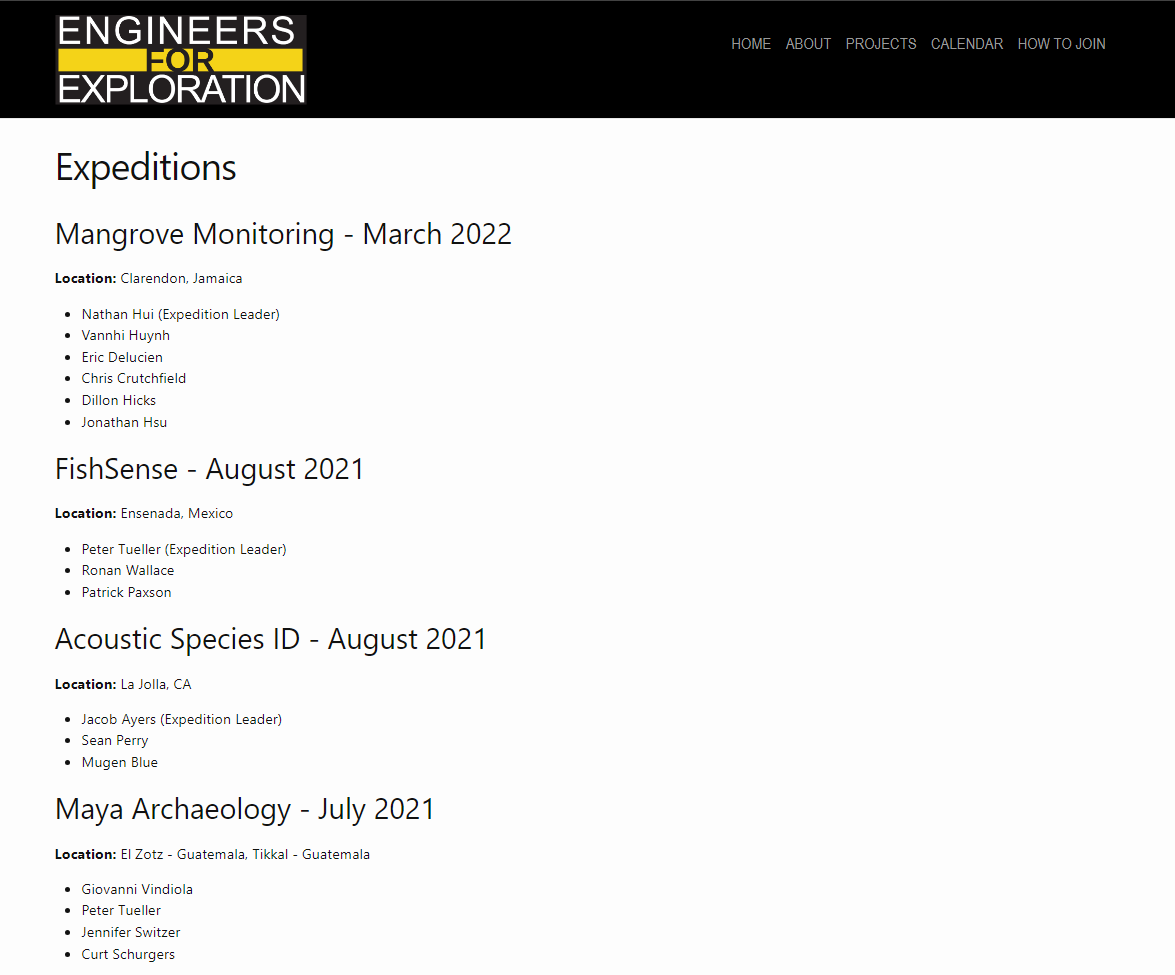
\includegraphics[height=0.7\textheight,width=0.7\textwidth,keepaspectratio]{./images/Screenshot 2024-04-29 123255.png}
\end{frame}
\begin{frame}{Projects (Phase 1) - Merged}
    \centering
    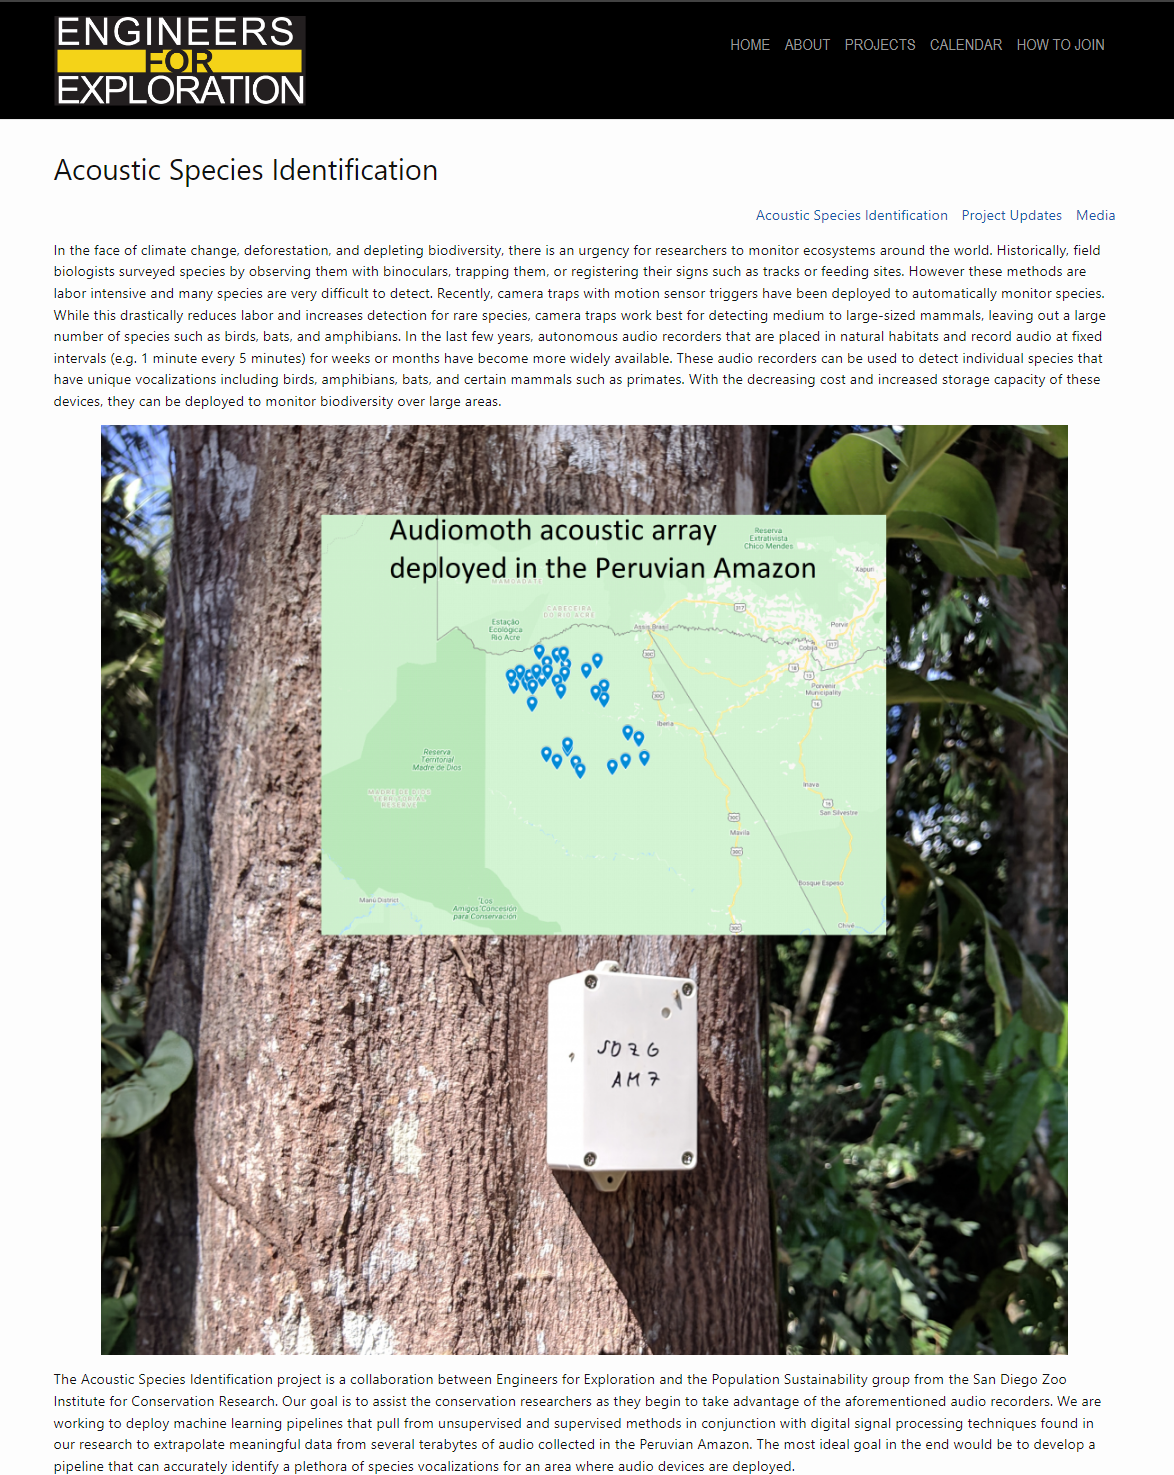
\includegraphics[height=0.7\textheight,width=0.7\textwidth,keepaspectratio]{./images/Screenshot 2024-04-29 123500.png}
\end{frame}
\begin{frame}{Photo Carousel - Merged (May Rework for Mobile)}
    \centering
    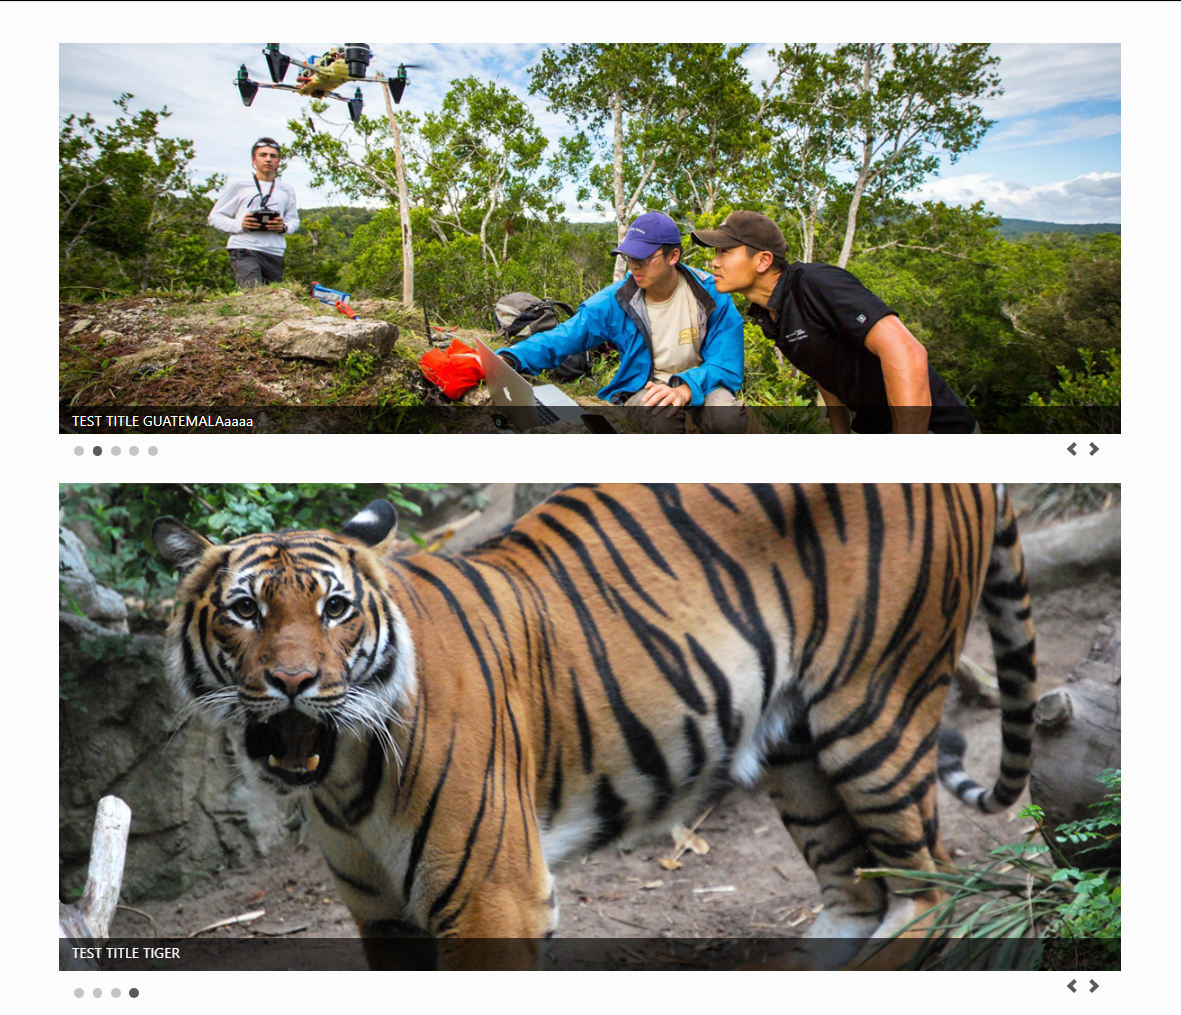
\includegraphics[height=0.7\textheight,width=0.7\textwidth,keepaspectratio]{./images/Screenshot 2024-04-29 123620.png}
\end{frame}
\begin{frame}{Director Photos - Merged}
    \centering
    
\includegraphics[height=0.7\textheight,width=0.7\textwidth,keepaspectratio]{./images/326290539-4b1b66e6-6d6f-4a5c-b453-96dc81ab773b.png}
\end{frame}
\begin{frame}{HomePage - In Progress}
    \centering
    
\includegraphics[height=0.7\textheight,width=0.7\textwidth,keepaspectratio]{./images/Screenshot 2024-05-06 102507.png}
\end{frame}
\begin{frame}{Techical Updates}
    \begin{itemize}
        \item WIP: New build config
        \item WIP: Custom image processing pipeline
        \item WIP: Rollout of project pages
    \end{itemize}
\end{frame}

% Slides for 2024-04-29
% To create a slide, use the following:
% \begin{frame}{TITLE}
%     BODY
% \end{frame}

% To create a slide with a bullet list, use the following:
% \begin{frame}{TITLE}
%     \begin{itemize}
%         \item ITEM 1
%         \item ITEM 2
%     \end{itemize}    
% \end{frame}

% To create a slide with numbered list, use the following:
% \begin{frame}{TITLE}
%     \begin{enumerate}
%         \item ITEM 1
%         \item ITEM 2
%     \end{enumerate}
% \end{frame}

% To create a slide with a graphic:
% 1. Add the graphic to this folder (named picture.png)
% 2. Use the following:
% \begin{frame}{TITLE}
%     \centering
%     \includegraphics[height=0.7\textheight,width=0.7\textwidth,keepaspectratio]{picture.png}
% \end{frame}

% To create a slide with two columns, use the following:
% \begin{frame}{TITLE}
%     \begin{columns}
%         \begin{column}{0.5\textwidth}
%             COLUMN 1 BODY
%         \end{column}
%         \begin{column}{0.5\textwidth}
%             COLUMN 2 BODY
%         \end{column}
%     \end{columns}
% \end{frame}
